%
% LaTeX report template 
%
\documentclass[a4paper,10pt]{article}
\usepackage{graphicx}
\usepackage{amsmath}
\usepackage{amssymb}
\usepackage[english]{babel}
\usepackage[latin1]{inputenc}
\usepackage[margin=1.25in]{geometry}
\graphicspath{{../img/}}

%
\begin{document}
%

   
   \title{{\large Universita' degli Studi di Padova \\ } {\normalsize Corso di laurea triennale in Ingegneria Informatica}\\ \vspace{1.8cm} \textbf{ Relazione 1\textsuperscript{a} simulazione SPICE}}

   \author{Giacomo Camposampiero, matricola 1187180}
          
   \date{20 novembre 2020}

   \maketitle
   
   \vspace{2.2cm}
   
   \renewcommand{\contentsname}{Indice}      
   \tableofcontents
   
   \newpage
  
\section{Esercizio primo}
Studio di un amplificatore audio con opamp commerciale LT1115, rappresentato in figura.
\begin{figure}[h!]
  	\centering
 	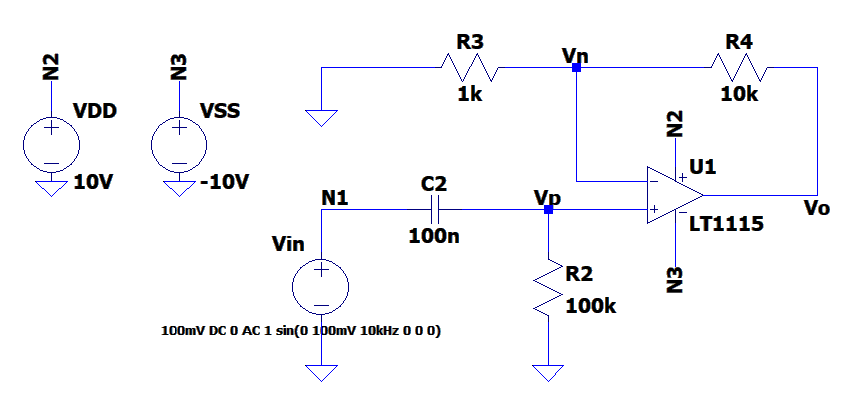
\includegraphics[width=0.7\linewidth]{ckt1.png}
  	\caption{Schema elettrico del circuito amplificatore.}
  	\label{fig:ckt1}
\end{figure}

\subsection{Calcolare analiticamente  il guadagno in tensione e la frequenza di taglio inferiore considerando l'amplificatore operazionale ideale}
Applicando il partitore di tensione al ramo in ingresso al morsetto positivo dell'amplificatore operazionale troviamo che
	\begin{align*}
      V_p = \frac{Z_2}{Z_1+Z_2}V_{in} = \frac{R_2}{R_2 + \frac{1}{sC_2}}V_{in} = \frac{sC_2R_2}{1+sC_2R_2}V_{in}
    \end{align*}
L'amplificatore operazionale e' utilizzato in configurazione non invertente. Dalla teoria, sappiamo che il guadagno in tensione di questa configurazione corrisponde a
	\begin{align*}
      A_v = 1+\frac{Z_4}{Z_3} = 1+\frac{R_4}{R_3}
    \end{align*}
Possiamo quindi concludere che il guadagno in tensione dell'amplificatore audio, considerando l'amplificatore operazionale ideale, e' regolato dalla funzione di trasferimento
	\begin{align*}
      W(s) = \frac{v_o(s)}{v_{in}(s)} =(1+\frac{Z_4}{Z_3})\cdot(\frac{Z_2}{Z_1+Z_2}) = (1+\frac{R_4}{R_3})\cdot(\frac{sC_2R_2}{1+sC_2R_2})
    \end{align*}
Riscriviamo la funzione di trasferimento in forma di Bode.
	\begin{align*}
      W(s) = \frac{K}{s^l}\cdot\frac{\prod\limits_{i=1}^{p}(1+sT)}{\prod\limits_{i=1}^{m}(1+s\tau)} = \frac{R_2C_2(R_3+R_4)}{R_3}\cdot\frac{1}{s^{-1}}\cdot\frac{1}{(1+sC_2R_2)}
    \end{align*}
Sostituendo alle costanti i valori numerici, troviamo infine che la frequenza di taglio e il guadagno ad alta frequenza dell'amplificatore corrispondono rispettivamente a
\begin{gather*}
	\omega_1 = \frac{1}{C_2R_2} = 10^2\frac{rad}{s} = 15.915Hz \\
	G_v = 1+\frac{R_4}{R_3} = 11\,(20.83dB)
\end{gather*}

\newpage
\subsection{Simulare la forma d'onda di uscita per un segnale sinusoidale di ingresso di 10 mV, a 1 Hz, 10 Hz, 10kHz}
Il listato SPICE utilizzato per simulare il circuito e' riportato di seguito. Il seguente codice e' stato utilizzato per simulare l'ingresso a 10kHz. Nelle altre simulazioni i valori di frequenza del segnale in ingresso e l'intervallo di tempo specificato nell'analisi del transitorio sono stati adattati di conseguenza.
\begin{quote}
\begin{verbatim}
* Esercizio 1.2
Vin N1 0 DC 0 AC 1 sin(0 10mV 10kHz 0 0 0)
VDD N2 0 10V
VSS N3 0 -10V
XU1 Vp Vn N2 N3 Vo LT1028
C2 Vp N1 100n
R2 Vp 0 100k
R4 Vn Vo 10k
R3 Vn 0 1k
.lib LTC.lib
.tran 0 0.3m
.backanno
.end
\end{verbatim}
\end{quote}
Di seguito sono riportate le forme d'onda in uscita ottenute a fronte di un ingresso con frequenza 1Hz (Figure \ref{fig:plot1hz}), 10Hz (Figure \ref{fig:plot10hz}) e 10kHz (Figure \ref{fig:plot10khz}).

\begin{figure}[h!]
	\centering
 	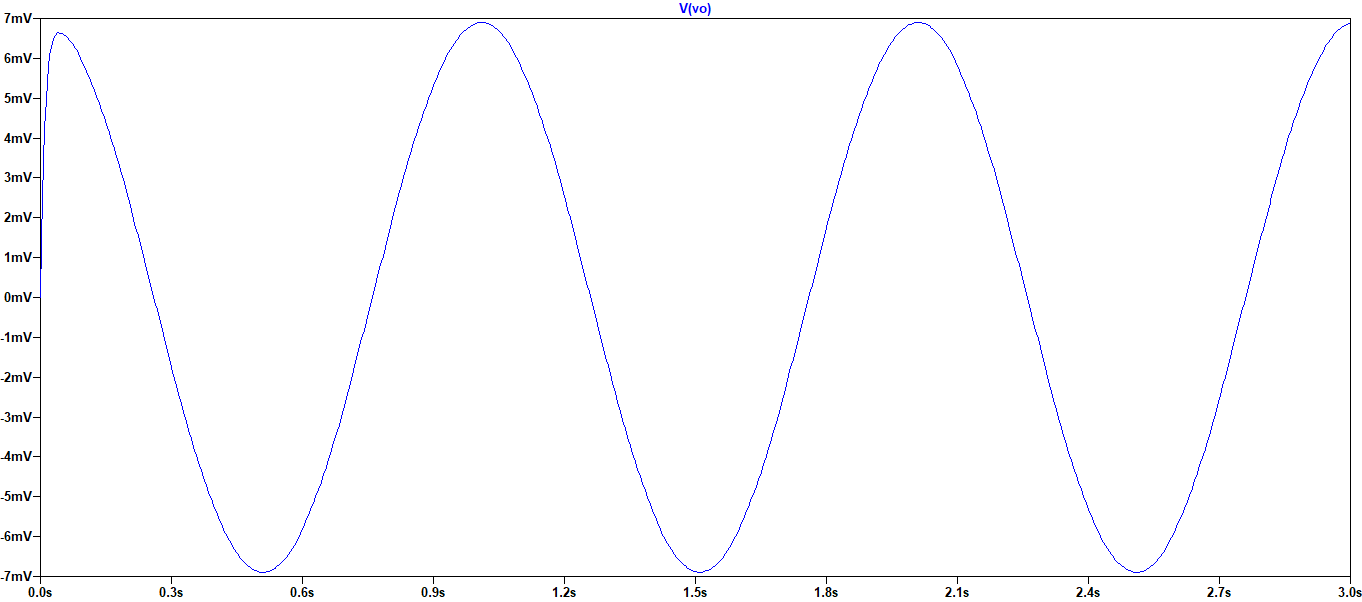
\includegraphics[width=0.8\linewidth]{plot1-2-1.png}
  	\caption{Ingresso a 1Hz.}
  	\label{fig:plot1hz}
\end{figure}

\begin{figure}[h!]
	\centering
 	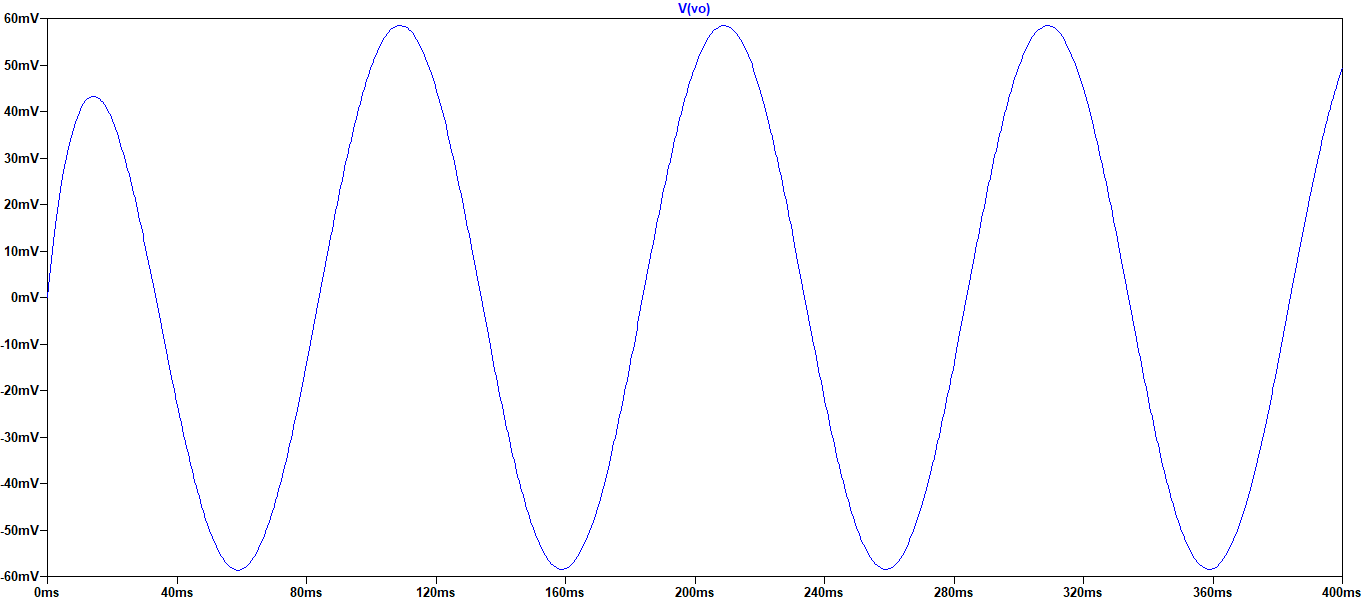
\includegraphics[width=0.8\linewidth]{plot1-2-2.png}
  	\caption{Ingresso a 10Hz.}
  	\label{fig:plot10hz}
\end{figure}

\begin{figure}[h!]
	\centering
 	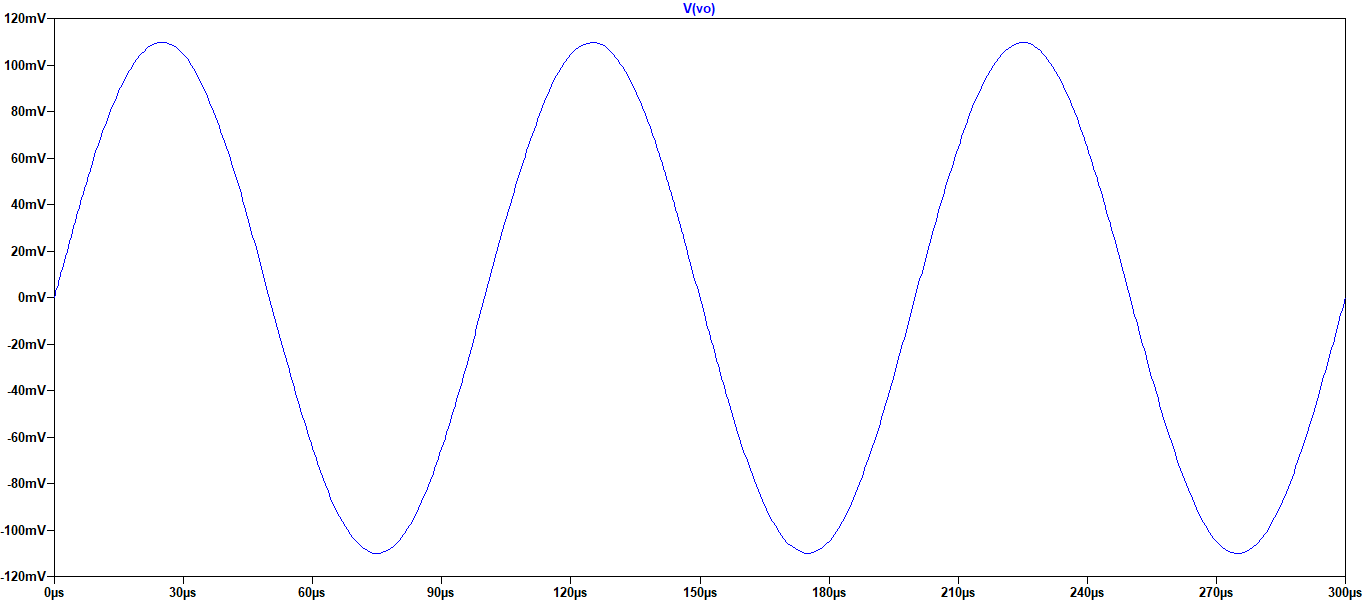
\includegraphics[width=0.8\linewidth]{plot1-2-3.png}
  	\caption{Ingresso a 10kHz.}
  	\label{fig:plot10khz}
\end{figure}

\subsection{Simulare il diagramma di Bode dell'ampiezza tra 1Hz e 100 kHz}
Per simulare il diagramma di Bode dell'ampiezza e' stato utilizzato il listato SPICE riportato di seguito. Il risultato dell'analisi in frequenza e' riportato graficamente (Figure \ref{fig:bode1}).
\begin{quote}
\begin{verbatim}
* Esercizio 1.3
Vin N1 0 DC 0 AC 1 sin(0 10mV 10kHz 0 0 0)
VDD N2 0 10V
VSS N3 0 -10V
XU1 Vp Vn N2 N3 Vo LT1028
C2 Vp N1 100n
R2 Vp 0 100k
R4 Vn Vo 10k
R3 Vn 0 1k
.lib LTC.lib
.ac DEC 10 1 100k
.backanno
.end
\end{verbatim}
\end{quote}

\begin{figure}[h!]
	\centering
 	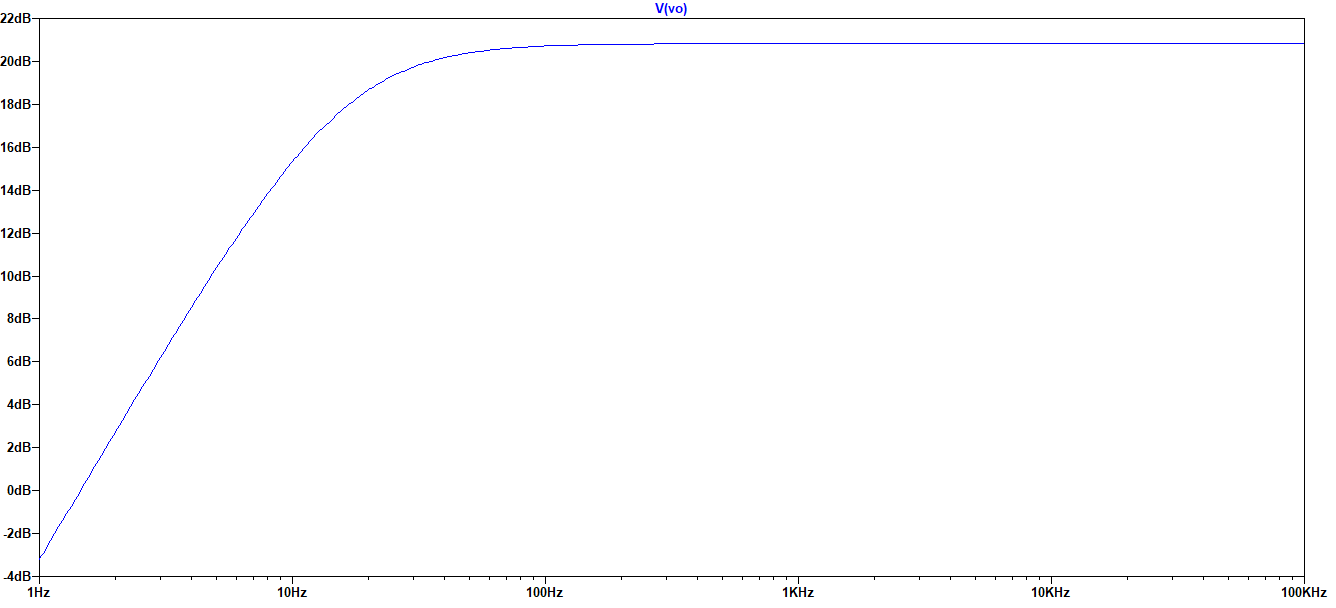
\includegraphics[width=1\linewidth]{plot1-3-1.png}
  	\caption{Diagramma di Bode dell'ampiezza tra 1Hz e 100kHz.}
  	\label{fig:bode1}
\end{figure}

\subsection{Per quale ampiezza del segnale di ingresso l'uscita satura? Simulare la forma  d'onda di uscita per un segnale di ingresso di ampiezza pari a 2 volte il valore trovato}
Innanzitutto, troviamo sperimentalmente l'ampiezza a cui satura l'amplificatore operazionale, fornendo al circuito segnali di svariate ampiezze e medesima frequenza (10kHz) in ingresso. Per fare cio', parametrizziamo l'ampiezza del segnale in ingresso e la facciamo variare a step di 200mV tra 100mV e 3V.
\small
\begin{quote}
\begin{verbatim}
* Esercizio 1.4
Vin N1 0 DC 0 AC 1 sin(0 {A} 10kHz 0 0 0)
VDD N2 0 10V
VSS N3 0 -10V
XU1 Vp Vn N2 N3 Vo LT1028
C2 Vp N1 100n
R2 Vp 0 100k
R4 Vn Vo 10k
R3 Vn 0 1k
.lib LTC.lib
.tran 0 0.5m
.step param A 100m 3 200m
.backanno
.end
\end{verbatim}
\end{quote}
\normalsize
\begin{figure}[h!]
	\centering
 	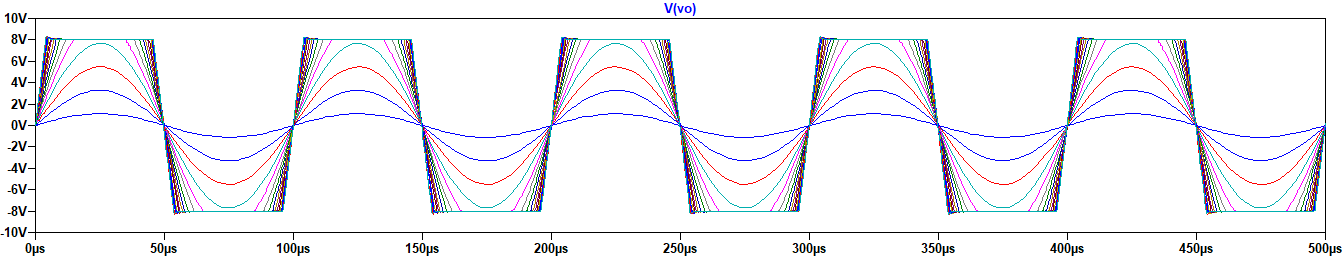
\includegraphics[width=1\linewidth]{plot1-4-1.png}
  	\caption{Forma d'onda in uscita al variare dell'ampiezza in ingresso.}
  	\label{fig:sat1}
\end{figure}
Dai risultati sperimentali si puo' dedurre che l'amplificatore satura ad un'ampiezza all'incirca pari a $8$V (se fosse ideale saturerebbe ad un'ampiezza in modulo di $10$V, ovvero la tensione di alimentazione in modulo fornita all'amplificatore operazionale). Troviamo analiticamente l'ampiezza del segnale in ingresso per cui appare il fenomeno di distorsione.
\begin{gather*}
	\lvert V_o \rvert\ = \lvert W(j\omega) \rvert\ \cdot \lvert V_{in} \rvert\ = \lvert \frac{2200j\pi}{1+200j\pi} \rvert\ \cdot \lvert V_{in} \rvert\ \\
	\Rightarrow \lvert V_{in} \rvert\ = \frac{8\cdot \sqrt{1+400\pi^2}}{2200\pi} = 0.727\,V
\end{gather*}
La forma d'onda del segnale di uscita, nel caso di un ingresso di ampiezza pari al doppio dell'ampiezza appena calcolata, e' riportata di seguito (Figure \ref{fig:sat2}).
    
\begin{figure}[h!]
	\centering
 	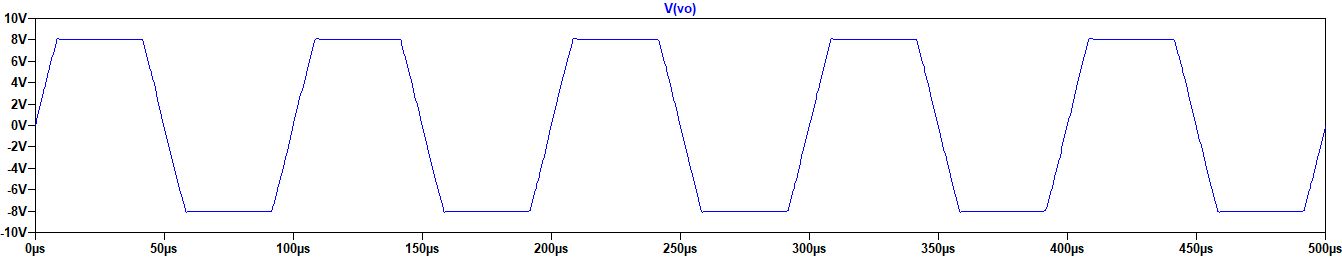
\includegraphics[width=1\linewidth]{plot1-4-2.png}
  	\caption{Forma d'onda in uscita con ingresso di ampiezza 1.45V.}
  	\label{fig:sat2}
\end{figure}

\subsection{Ripetere sostituendo a R2 una resistenza di valore pari al vostro numero di matricola diviso 100}
Sostituendo al valore della resistenza R2 il mio numero di matricola diviso 100 (R2 = 11871.8$\Omega$) i risultati ottenuti nei punti precedenti cambiano di conseguenza. La frequenza di taglio viene ricalcolata di seguito, mentre il guadagno ad altra frequenza rimane invariato in quanto indipendente da R2.
\begin{align*}
\omega_1 = \frac{1}{C_2R_2} = 842.33 \frac{rad}{s} = 134.06Hz
\end{align*}
Per quanto riguarda le nuove forme d'onda in uscita alle diverse frequenze (1Hz, 10Hz e 10kHz), i nuovi grafici sono rappresentati nelle figure Figure \ref{fig:plot1hzr2}, Figure \ref{fig:plot10hzr2} e Figure \ref{fig:plot10khzr2}. Il diagramma di Bode tra le frequenze di 1Hz e 100kHz aggiornato diventa quello rappresentato in figura Figure \ref{fig:plotboder2}.
\begin{figure}[h!]
	\centering
 	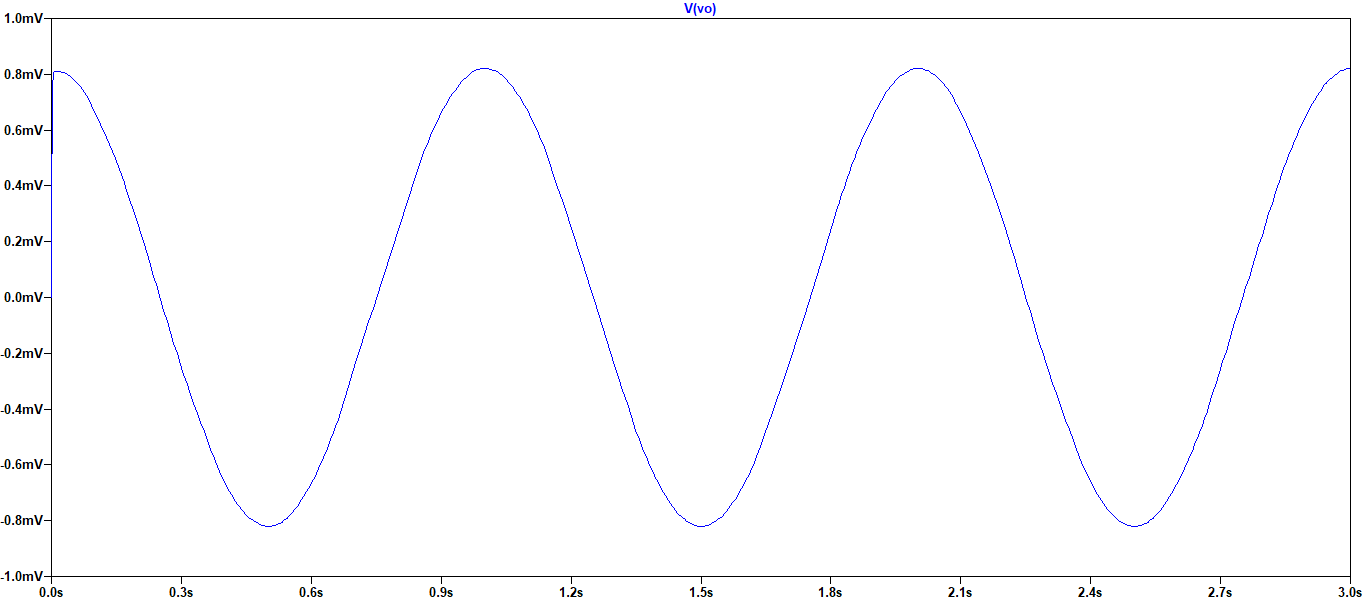
\includegraphics[width=0.6\linewidth]{plot1-5-1.png}
  	\caption{Ingresso a 1Hz con valore di resistenza R2 aggiornato.}
  	\label{fig:plot1hzr2}
\end{figure}

\begin{figure}[h!]
	\centering
 	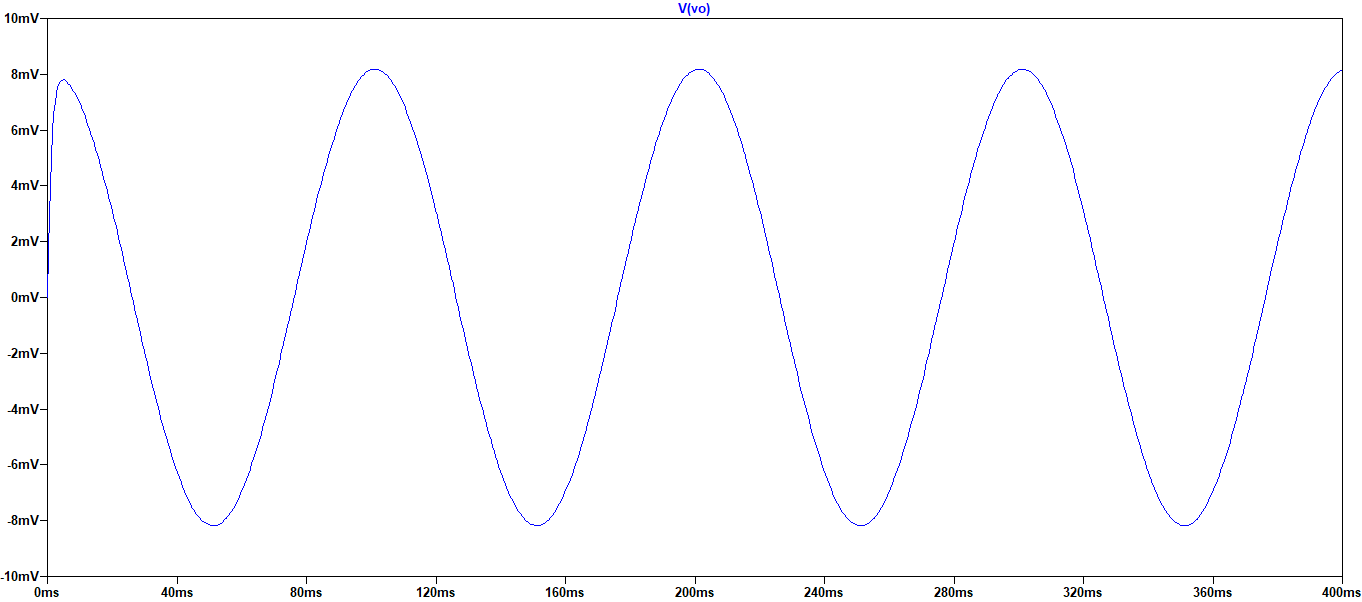
\includegraphics[width=0.6\linewidth]{plot1-5-2.png}
  	\caption{Ingresso a 10Hz con valore di resistenza R2 aggiornato.}
  	\label{fig:plot10hzr2}
\end{figure}

\begin{figure}[h!]
	\centering
 	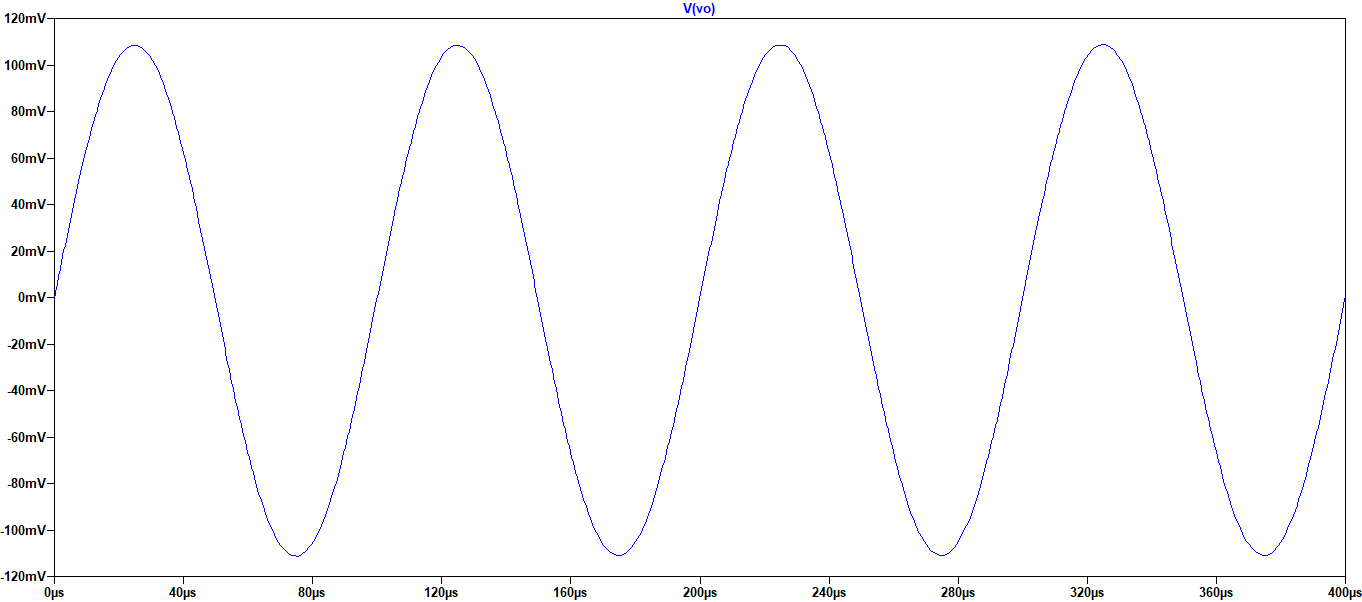
\includegraphics[width=0.6\linewidth]{plot1-5-3.png}
  	\caption{Ingresso a 10kHz con valore di resistenza R2 aggiornato.}
  	\label{fig:plot10khzr2}
\end{figure}

\begin{figure}[h!]
	\centering
 	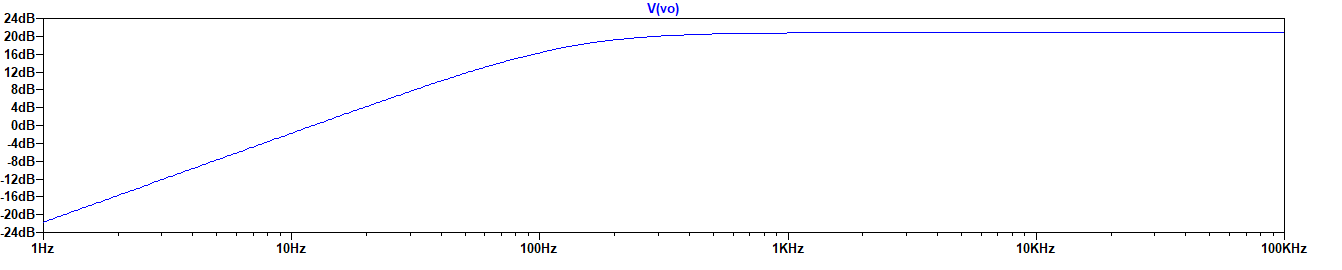
\includegraphics[width=1\linewidth]{plot-1-5-bode.png}
  	\caption{Diagramma di Bode con valore di resistenza R2 aggiornato.}
  	\label{fig:plotboder2}
\end{figure}

\pagebreak
Per quanto riguarda la saturazione, infine, ripetiamo la ricerca sperimentale dell'ampiezza massima a cui satura il segnale in uscita (con lo stesso listato SPICE del punto 1.4, in cui viene sostituito solamente il valore della resistenza R2). Il risultato e' riportato in figura Figure \ref{fig:plotsatr2}.

\begin{figure}[h!]
	\centering
 	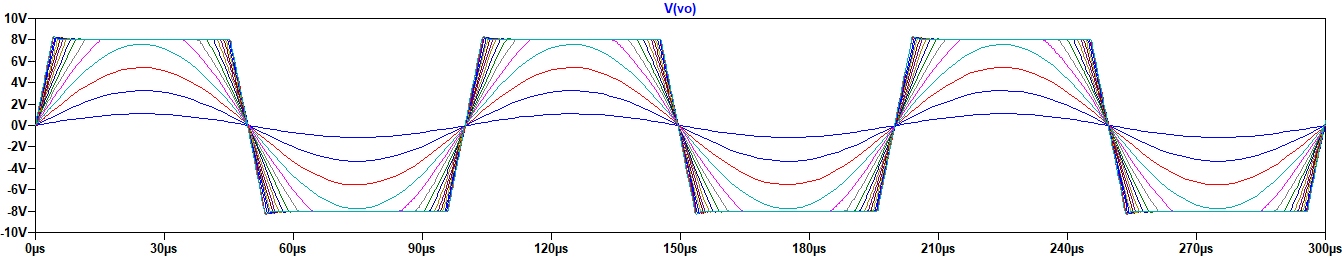
\includegraphics[width=1\linewidth]{plot-1-5-sat.png}
  	\caption{Ricerca sperimentale dell'ampiezza a cui satura l'amplificatore.}
  	\label{fig:plotsatr2}
\end{figure}

Successivamente, ricalcoliamo analiticamente l'ampiezza del segnale in ingresso per cui l'amplificatore satura e riportiamo la forma d'onda del segnale in uscita a fronte di un ingresso di ampiezza doppia rispetto a quella trovata algebricamente.
\begin{align*}
\lvert V_o \rvert\ = \lvert W(j\omega) \rvert\ \cdot \lvert V_{in} \rvert\ \Rightarrow \lvert V_{in} \rvert\ = 0.737\,V
\end{align*}
Il grafico della forma d'onda in uscita a fronte di un segnale in ingresso di ampiezza pari al doppio dell'ampiezza appena calcolata e' riportato di seguito (Figure \ref{fig:plottaglior2}).
\begin{figure}[h!]
	\centering
 	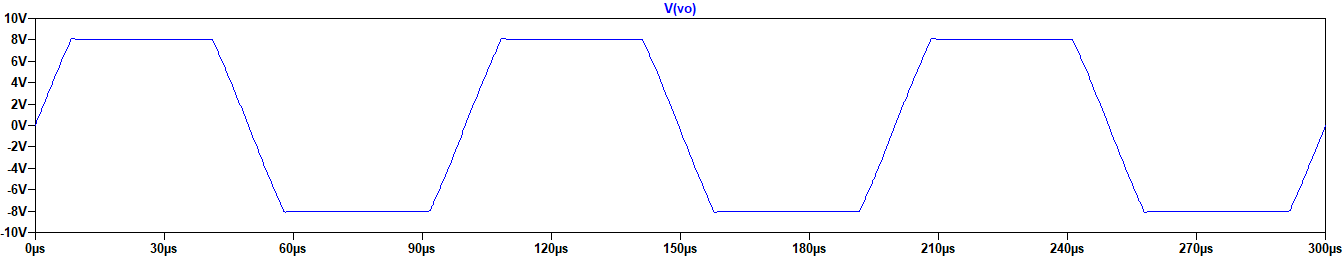
\includegraphics[width=1\linewidth]{plot-1-5-sat2.png}
  	\caption{Forma d'onda del segnale in uscita con ampiezza doppia rispetto a quella calcolata.}
  	\label{fig:plottaglior2}
\end{figure}

\newpage

\subsection{Qual e' la potenza assorbita dall'alimentazione nei due casi?}
La potenza assorbita dall'amplificatore operazionale corrisponde alla somma delle potenze erogate dai due generatori con cui e' alimentato l'amplificatore operazionale stesso. Quest'ultima puo' essere calcolata come
\begin{align*}
P_{out, alimentazione} = V_{ss} \cdot I_{ss} + V_{dd} \cdot I_{dd}
\end{align*}
Misurando questa grandezza, troviamo la potenza erogata dall'alimentazione per i due diversi valori di resistenza R2 100k$\Omega$ e 11871.8$\Omega$ (rispettivamente Figure \ref{fig:pow1} e Figure \ref{fig:pow2}).

\begin{figure}[h!]
	\centering
 	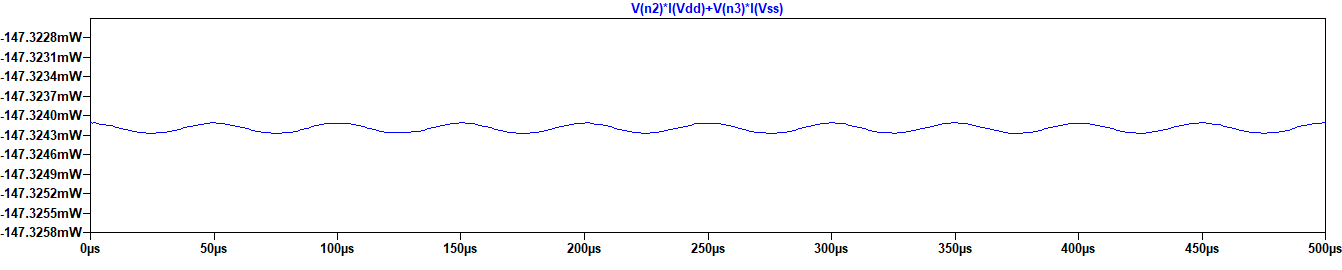
\includegraphics[width=1\linewidth]{plot1-6-norm.png}
  	\caption{Resistenza R2 pari a 100k$\Omega$.}
  	\label{fig:pow1}
\end{figure}

\begin{figure}[h!]
	\centering
 	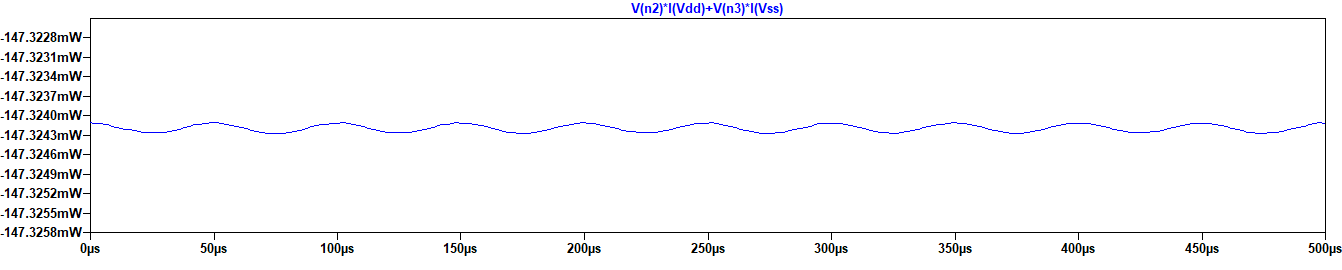
\includegraphics[width=1\linewidth]{plot1-6-mod.png}
  	\caption{Resistenza R2 pari a 11\,871.8$\Omega$.}
  	\label{fig:pow2}
\end{figure}

Possiamo notare come non sia visibile (per questi valori di resistenza) una dipendenza evidente della potenza erogata dal valore della resistenza R2. Inoltre, la potenza del grafico e' negativa, in quanto espressa secondo la convenzione degli utilizzatori (potenze minori di 0 equivalgono a potenze erogate).

\pagebreak

\section{Esercizio secondo}
Il generatore di corrente I1 e' un elemento termosensibile (nome commerciale AD590) che genera una corrente pari a 1$\mu$A per grado Kelvin. Quindi a 0$^{\circ}$C la corrente I1 = 273$\mu$A; a 100$^{\circ}$C e' 373$\mu$A.
Si vuole realizzare con questo sensore un termometro (convertitore temperatura-tensione) che fornisca una tensione di uscita di 10 mV/$^{\circ}$C.
\begin{figure}[h!]
	\centering
 	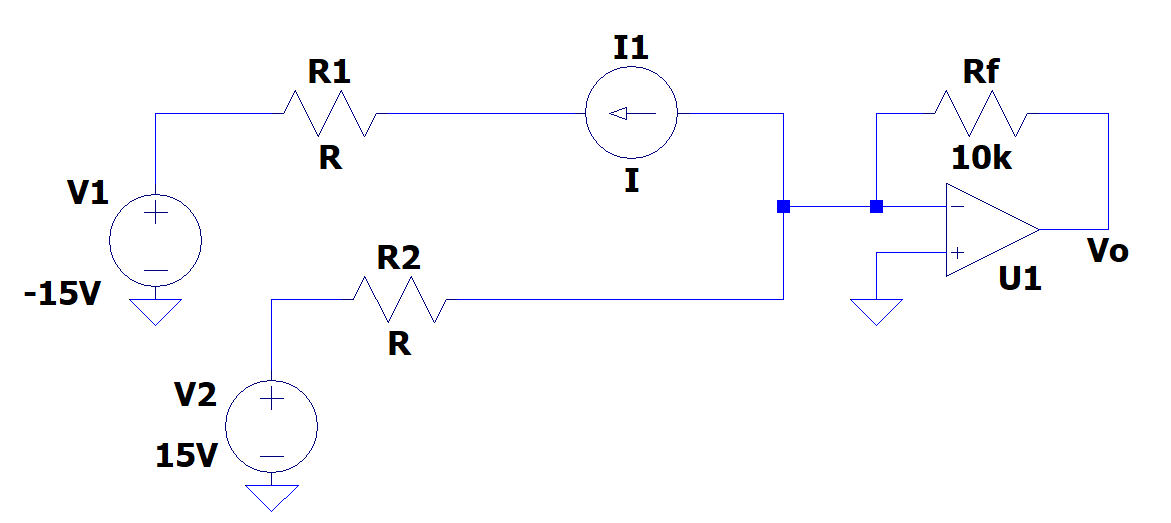
\includegraphics[width=0.7\linewidth]{ckt2.png}
  	\caption{Schema del circuito elettrico.}
  	\label{fig:ckt2}
\end{figure}

\subsection{Dato il valore di R1, trovare il valore di R2 che permette di ottenere il fattore di conversione desiderato}
Il valore di R1 dato corrisponde a $R1=10k\Omega$. Definiamo le correnti $I_1$, $I_2$ e $I_f$, corrispondenti alle correnti che scorrono nel ramo di V1, V2 e retroazione. Il parametro T utilizzato nelle seguenti relazioni rappresenta la temperatura in gradi Kelvin. Per il principio di massa virtuale, sappiamo che il morsetto negativo dell'ompamp e' a massa. 
\begin{gather*}
I_1 = T \cdot 1\mu A \\
I_2 = \frac{15V}{R_2} 
\end{gather*}
Dalla teoria, sappiamo che il morsetto negativo dell'ompamp non assorbe corrente. Per la legge di Kirchhoff delle correnti, quindi, la corrente $I_f$ puo' essere calcolata come
\begin{align*}
I_f = I_2 - I_1 = \frac{15V}{R2} - T\cdot 1\mu A
\end{align*}

La tensione in uscita $V_o$ puo' quindi essere calcolata come caduta di tensione sulla resistenza $R_f$ per effetto della corrente $I_f$. 
\begin{align*}
V_o = -I_f \cdot R_f = (T\cdot 1\mu A - \frac{15V}{R2}) \cdot R_f = T\cdot 10mV - \frac{150kV}{R2}
\end{align*}
Sapendo che ad una temperatura di $0^{\circ}$ Celsius l'output del circuito deve essere nullo, possiamo trovare il valore di $R2$ di conseguenza.
\begin{align*}
2.73 - \frac{150kV}{R_2} = 0 \Rightarrow R_2 = \frac{150\cdot 10^3}{2.73} \simeq 54\,945k\Omega
\end{align*}

\pagebreak

\subsection{Sostituite a Rf il vostro numero di matricola diviso per 100 e modificare il circuito in modo da ottenere 10mV/grado Celsius in uscita}
Sostituita $R_f$ con una resistenza equivalente al mio numero di matricola diviso 100, la relazione che governa l'andamento dell'uscita in tensione $V_o$ del circuito diventa
\begin{align*}
V_o = (T\cdot 10^{-6}A - \frac{15V}{R2})\cdot 1,18718\cdot 10^4 \Omega
\end{align*}
Con questo nuovo valore di resistenza, troviamo che sia il coefficiente angolare che il termine noto dell'equazione devono essere corretti affinche' il circuito ritorni ad essere coerente con il comportamento lineare definito inizialmente.  \par

Per correggere il coefficiente angolare della retta, che rappresenta il guadagno in mV per ogni grado Celsius del circuito, e' necessario correggere la corrente $I_1$ che arriva al nodo su cui precedentemente abbiamo applicato la legge di Kirchhoff delle correnti. Modifichiamo il circuito di aggiungendo due resistenze $R_{p1}=1871.8\Omega$ e $R_{p2}=10k\Omega$ (Figure \ref{fig:ckt2mod}).
\begin{figure}[h!]
	\centering
 	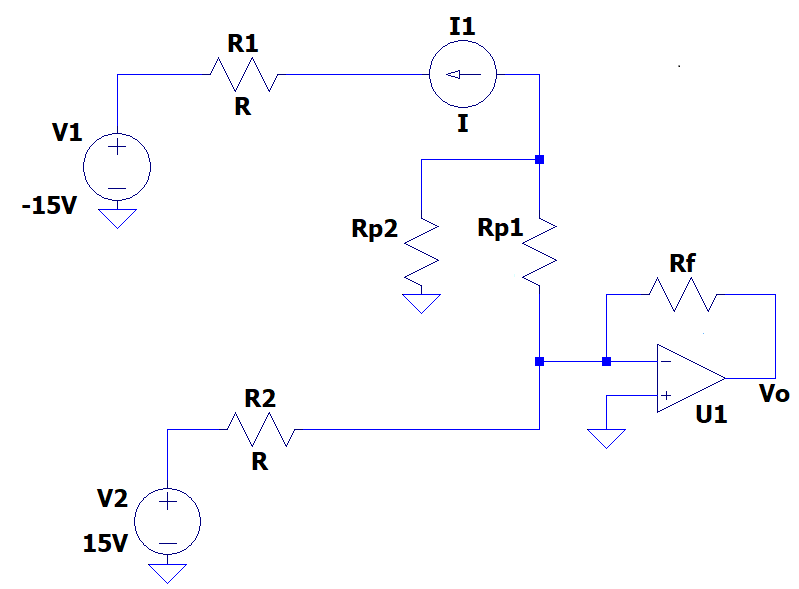
\includegraphics[width=0.5\linewidth]{ckt2-2.png}
  	\caption{Schema elettrico del circuito modificato.}
  	\label{fig:ckt2mod}
\end{figure}
\par
In questo modo creiamo un partitore di corrente per $I_1$ sulle resistenze $R_{p1}$ ed $R_{p2}$ (che per il principio di massa virtuale si trovano in parallelo). La corrente $I_1'$ in ingresso al nodo su cui abbiamo precedentemente applicato Kirchhoff per le correnti diventa
\begin{align*}
I_1' =\frac{R_{p2}}{R_{p1}+R_{p2}} I_1 = \frac{10k\Omega}{10k\Omega+1871.8\Omega}I_1 = \frac{1}{1.18718}I_1
\end{align*} 
Di conseguenza, la relazione legge che regola la tensione in uscita $V_o$ diventa
\begin{align*}
V_o=(\frac{1}{1.18718}T\cdot10^{-6}A-\frac{15V}{R_2})\cdot 1.18718\cdot10^4\Omega = T\cdot10mV- \frac{178\,077}{R_2} 
\end{align*}
Calcolando come prima la relazione per 0$^{\circ}$C nell'incognita $R_2$, siamo in grado di trovare il valore di quest'ultima.
\begin{align*}
R_2 = \frac{178\,077}{2.73} \simeq 65\,230 \Omega
\end{align*}
\pagebreak

\subsection{Scrivere il listato SPICE .cir del circuito, commentarlo; definire I1 come generatore di corrente comandato da un parametro "temperatura". Graficare la tensione di uscita simulata da SPICE nell'intervallo da 0 a 100 gradi Celsius}
Il listato SPICE utilizzato per simulare il circuito e' riportato di seguito.
\small
\begin{verbatim}
* Esercizio 2.3
R1 N2 N1 10k
R2 N3 N4 54945
* Generatori di tensione
V1 N1 0 -15V
V2 N4 0 15V
* Generatore di corrente "pilotato" dal parametro temperatura
I1 N3 N2 {temperatura*1u}
Eopamp Vo 0 0 N3 1000000
Rf Vo N3 10k
* Richiesta di analisi sulla variazione del parametro temperatura
.dc param temperatura 273 373 1
.backanno
.end
\end{verbatim}
\normalsize
Nel caso di resistenza $R_f$ uguale al mio numero di matricola diviso 100, il listato .cir e' modificato nel seguente modo, sulla base dei risultati ottenuti nel punto 2.2.
\small
\begin{verbatim}
* Esercizio 2.3
R1 N2 N1 10k
R2 N3 N4 65230
* Resistenze parallelo aggiunto
Rp1 N3 Np 1871.8
Rp2 0 Np 10k
* Generatori di tensione
V1 N1 0 -15V
V2 N4 0 15V
* Generatore di corrente "pilotato" dal parametro temperatura
I1 Np N2 {temperatura*1u}
Eopamp Vo 0 0 N3 1000000
Rf Vo N3 11871.8
* Richiesta di analisi sulla variazione del parametro temperatura
.dc param temperatura 273 373 1
.backanno
.end
\end{verbatim} 
\normalsize
Il grafico della tensione in uscita in funzione della temperatura T in input espressa in Kelvin risulta lo stesso in entrambi i casi ed e' riportato di seguito (Figure \ref{fig:tensionetemper}). 
\begin{figure}[h!]
	\centering
 	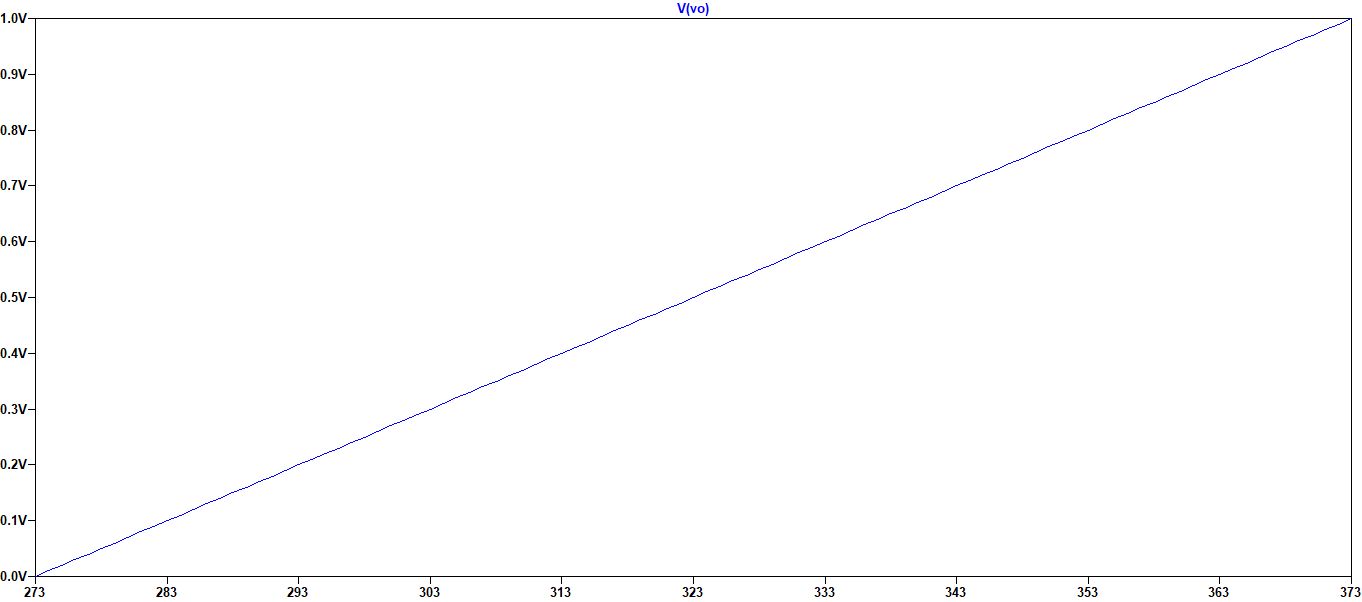
\includegraphics[width=0.7\linewidth]{plot1-2-5.png}
  	\caption{Grafico tensione in uscita/temperatura in gradi Kelvin.}
  	\label{fig:tensionetemper}
\end{figure}


\pagebreak
\section{Esercizio terzo}
Studio di un filtro RC (numero di matricola che termina con 0) rappresentato in figura.
\begin{figure}[h!]
	\centering
 	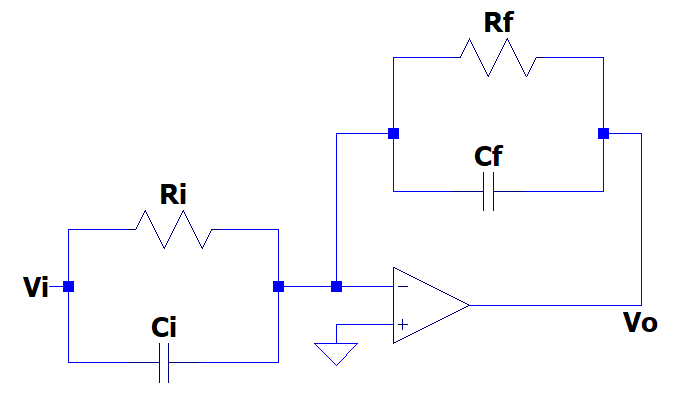
\includegraphics[width=0.5\linewidth]{ckt3.png}
  	\caption{Schema elettrico del circuito.}
  	\label{fig:ckt3}
\end{figure}

\subsection{Dimostrare che la funzione di trasferimento del circuito e' quella riportata nella tabella}
Dimostro che la funzione di trasferimento del circuito e'
\begin{align*}
W(s) = -\frac{R_f}{R_i} \cdot \frac{1+sR_1C_1}{1+sR_fC_f}
\end{align*}
Per prima cosa, notiamo che l'amplificatore e' utilizzato in configurazione invertente. Dalla teoria sappiamo che il guadagno di questa configurazione corrisponde ad
\begin{align*}
A = -\frac{Z_f}{Z_i}
\end{align*}
Calcoliamo il valore delle due impedenze, $Z_i$ e $Z_f$.
\begin{gather*}
Z_i = R_i \parallel C_i = \frac{R_i}{1+sC_iR_i} \\
Z_f = R_f \parallel C_f = \frac{Rf}{1+sC_fR_f}
\end{gather*}
La funzione di trasferimento puo' essere quindi riscritta come
\begin{align*}
W(s) = -\frac{Z_f}{Z_i} = -\frac{R_f}{1+sC_fR_f} \cdot \frac{1+sC_iR_i}{R_i} = -\frac{R_f}{R_i} \cdot \frac{1+sC_iR_i}{1+sC_fR_f}\qquad  \blacksquare
\end{align*}
\pagebreak

\subsection{Simulare con SPICE il diagramma di Bode dell'ampiezza e della fase, sostituiti i valori di resistenza e capacita' con i valori dati.}
Sostituiamo i valori di resistenze e capacita' con i valori dati $R_i=1k\Omega$, $C_i=100nF$, $R_f=100k\Omega$ e $C_f=1 \mu F$. Il listato del circuito corrisponde e' riportato di seguito. Nel listato il modello di opamp ideale della libreria opamp.sub e' stato sostituito da un generatore di tensione comandato in tensione VCVS, in cui il fattore di proporzionalita' e' stato fissato a $10^6$ per approssimare un guadagno infinito.
\begin{verbatim}
* Esercizio 3.2
Vin Vi 0 DC 0 AC 1 sin(0 100m 10kHz 0 0 0)
Ci N1 Vi 100n
Cf Vo N1 1u
Ri N1 Vi 1k
Rf Vo N1 100k
Eopamp Vo 0 0 N1 1000000
.ac dec 10 0.1 100k
.backanno
.end
\end{verbatim}    	
Il diagramma di Bode di fase e ampiezza e' riportato di seguito (Figure \ref{fig:bode3}). I risultati sono coerenti con quelli che e' possibile calcolare analiticamente a partire dalla funzione di trasferimento W(s). 

\begin{figure}[h!]
	\centering
 	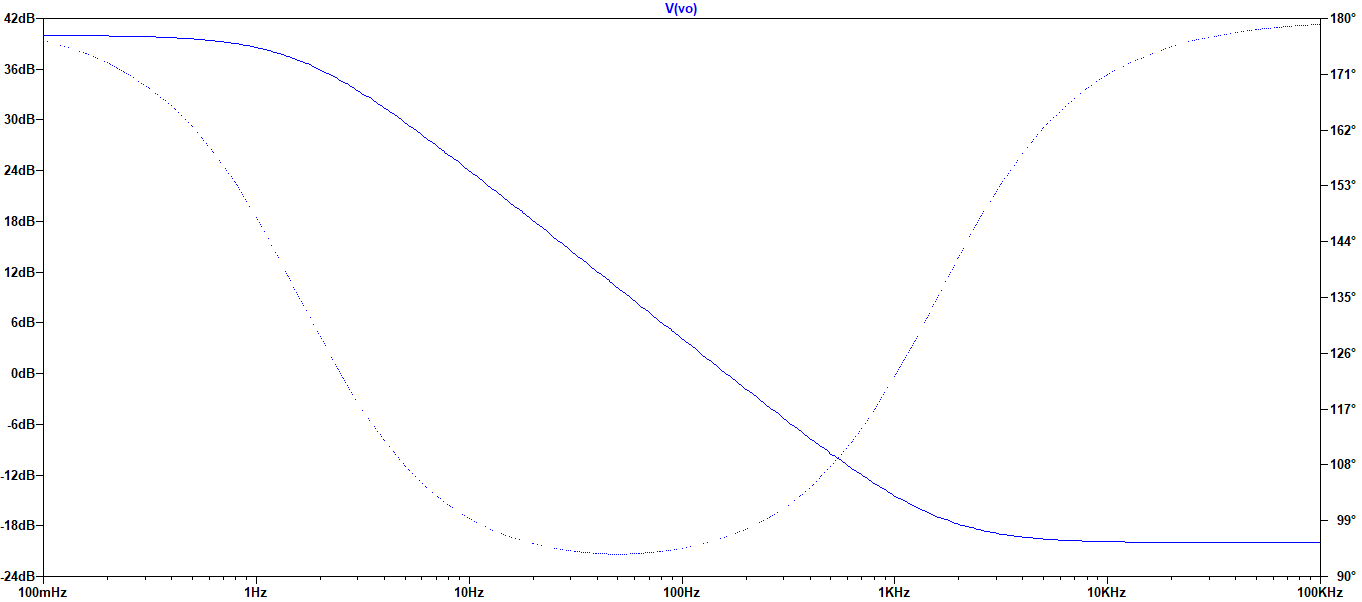
\includegraphics[width=1\linewidth]{plot3-1.png}
  	\caption{Diagramma di Bode di fase e ampiezza.}
  	\label{fig:bode3}
\end{figure}
\pagebreak

\subsection{Simulare con SPICE il segnale di uscita corrispondente ad un ingresso sinusoidale di ampiezza 100 mV con frequenza di 100Hz; 1kHz; 10kHz; 10MHz}
Per simulare la forma d'onda del segnale di uscita viene utilizzato il listato SPICE riportato di seguito. Il valore della frequenza viene fatto variare manualmente ad ogni simulazione; il gap tra frequenze non permette infatti di visualizzare correttamente tutti gli output contemporaneamente. I grafici delle forme d'onda in uscita sono riportati di seguito. Le "curve" che si possono notare a basse frequenze sono dovute probabilmente ad effetti capacitivi del circuito. 
\begin{verbatim}
* Esercizio 3.3
Vin Vi 0 DC 0 AC 1 sin(0 100mV 10k 0 0 0)
Ci N1 Vi 100n
Cf Vo N1 1u
Ri N1 Vi 1k
Rf Vo N1 100k
Eopamp Vo 0 0 N1 1000000
.tran 0 0.5m
.backanno
.end
\end{verbatim}

\begin{figure}[h!]
	\centering
 	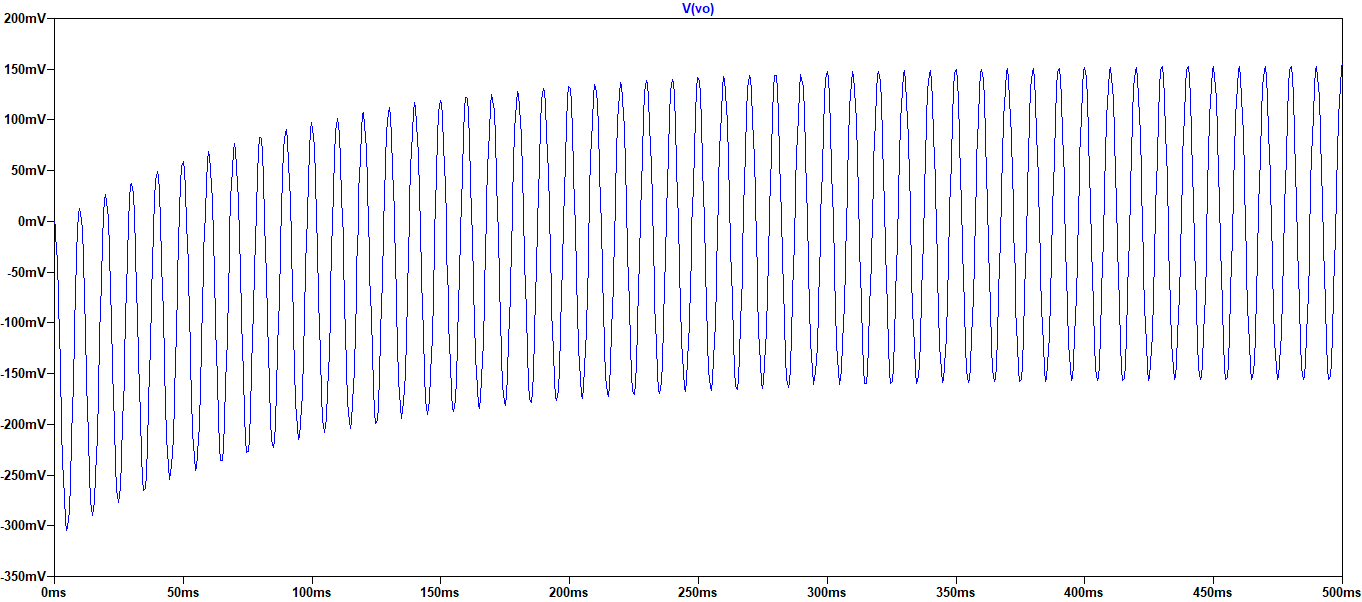
\includegraphics[width=1\linewidth]{plot3-100.png}
  	\caption{Segnale in ingresso di frequenza 100Hz.}
  	\label{fig:out100}
\end{figure}
\begin{figure}[h!]
	\centering
 	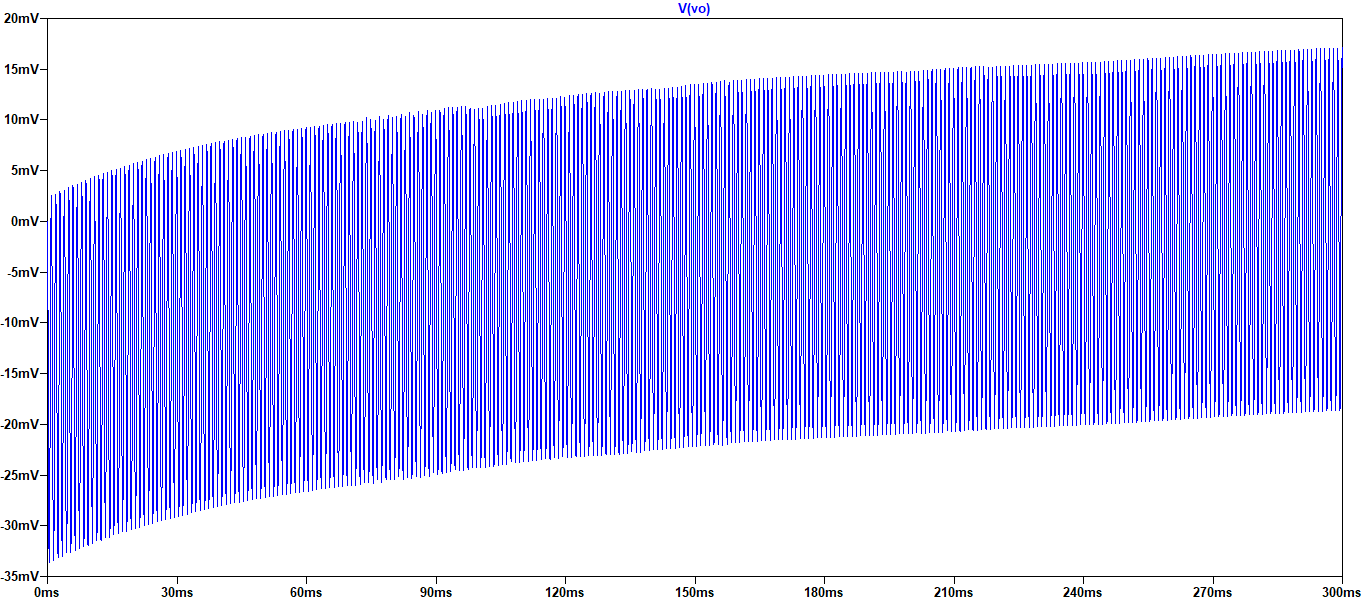
\includegraphics[width=1\linewidth]{plot3-1k.png}
  	\caption{Segnale in ingresso di frequenza 1kHz.}
  	\label{fig:out1k}
\end{figure}
\begin{figure}[h!]
	\centering
 	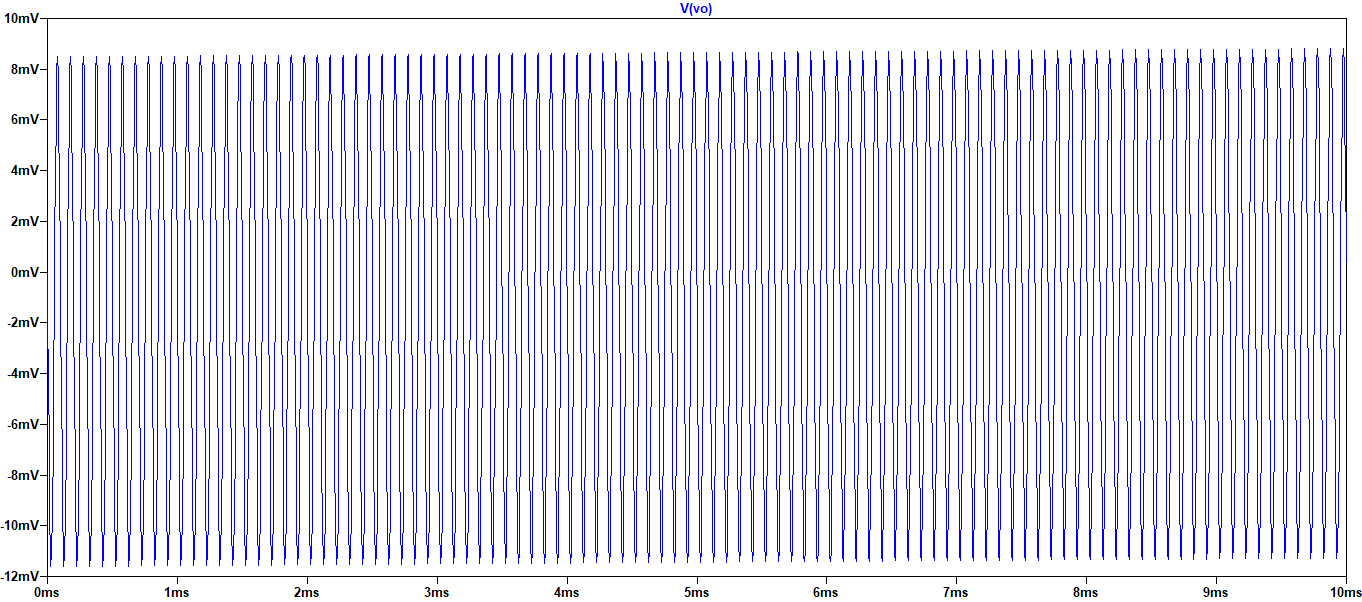
\includegraphics[width=1\linewidth]{plot3-10k.png}
  	\caption{Segnale in ingresso di frequenza 10kHz.}
  	\label{fig:out100k}
\end{figure}
\begin{figure}[h!]
	\centering
 	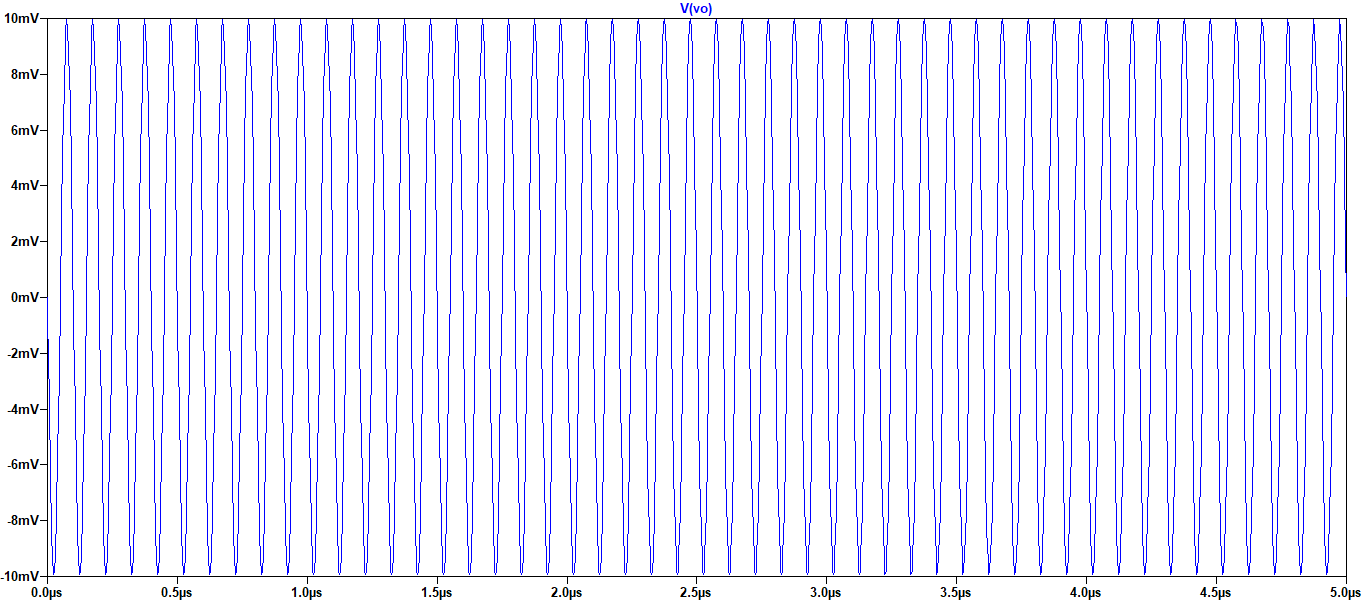
\includegraphics[width=1\linewidth]{plot3-10M.png}
  	\caption{Segnale in ingresso di frequenza 10MHz.}
  	\label{fig:out10meg}
\end{figure}

\end{document}